\documentclass[border=3pt,tikz]{standalone}
% Shared look for every TikZ figure in these notes.
% Included by each standalone figure file; also keeps the figures consistent
% with the colours used in the PDF and on the website.

\usepackage{tikz}
\usepackage{pgfplots}
\pgfplotsset{compat=1.18}
\usetikzlibrary{arrows.meta, decorations.markings, decorations.pathmorphing,
                patterns, calc, positioning}
\usepackage{amsmath}

% Series colours are the three validated categorical slots also used by the
% interactive widgets, so a path drawn in the printed notes and the same path on
% the website are the same colour. They clear the colour-vision-deficiency and
% contrast checks as a set; every path is direct-labelled as well, so colour is
% never the only thing carrying identity.
\definecolor{duPurple}{HTML}{68246D}
\definecolor{duBlue}{HTML}{2A78D6}
\definecolor{duRed}{HTML}{EB6834}
\definecolor{duGreen}{HTML}{1BAF7A}
\definecolor{duGrey}{HTML}{6B6B6B}

\tikzset{
  axisline/.style   = {-{Stealth[length=3mm]}, line width=0.7pt, black},
  path1/.style      = {duBlue,   line width=1.1pt},
  path2/.style      = {duRed,    line width=1.1pt},
  path3/.style      = {duGreen,  line width=1.1pt},
  statedot/.style   = {circle, fill=black, inner sep=1.4pt},
  arrowhead/.style  = {decoration={markings,
                        mark=at position #1 with {\arrow{Stealth[length=2.6mm]}}},
                       postaction={decorate}},
  lbl/.style        = {font=\small},
  slbl/.style       = {font=\footnotesize, duGrey},
  workfill/.style   = {duPurple, opacity=0.16},
}

\begin{document}
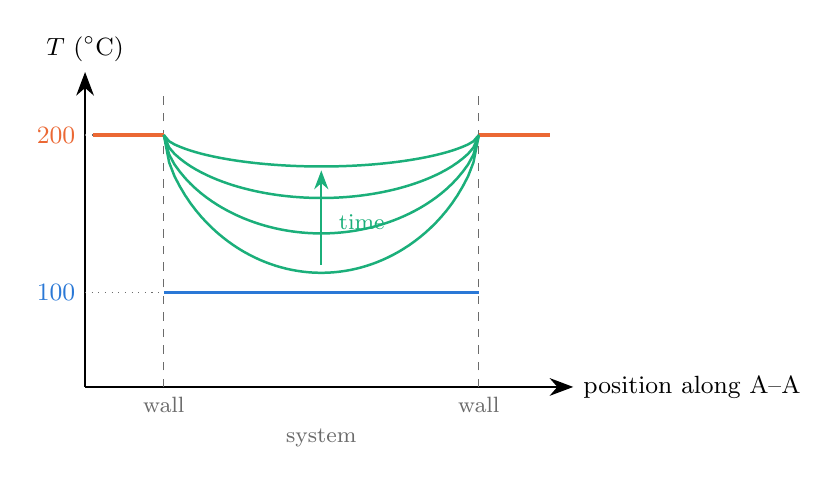
\begin{tikzpicture}
  % temperature across section A--A of the system, while it heats up
  \draw[axisline] (0,0) -- (6.2,0) node[right, lbl] {position along A--A};
  \draw[axisline] (0,0) -- (0,4.0) node[above, lbl] {$T$ ($^\circ$C)};
  \draw[duGrey, dashed, line width=0.4pt] (1.0,0) -- (1.0,3.7);
  \draw[duGrey, dashed, line width=0.4pt] (5.0,0) -- (5.0,3.7);
  \node[slbl, below] at (1.0,0) {wall};
  \node[slbl, below] at (5.0,0) {wall};
  \node[slbl] at (3.0,-0.65) {system};
  % source at 200 C outside the system
  \draw[path2] (0.1,3.2) -- (1.0,3.2);
  \draw[path2] (5.0,3.2) -- (5.9,3.2);
  \node[lbl, duRed, left] at (0,3.2) {200};
  % initial uniform 100 C
  \draw[path1] (1.0,1.2) -- (5.0,1.2);
  \node[lbl, duBlue, left] at (0,1.2) {100};
  \draw[duGrey, dotted] (0,1.2) -- (1.0,1.2);
  \draw[duGrey, dotted] (0,3.2) -- (0.1,3.2);
  % intermediate profiles: hot near the walls, cooler in the middle
  \foreach \d in {1.75,1.25,0.8,0.4} {
    \draw[path3, line width=0.9pt] plot[domain=1.0:5.0, samples=60]
      (\x, {3.2 - \d*(1 - ((\x-3.0)/2.0)^2)^0.6 - (2.0-\d)*0});
  }
  \draw[-{Stealth[length=2.4mm]}, duGreen, line width=0.7pt] (3.0,1.55) -- (3.0,2.75);
  \node[slbl, duGreen, right, align=left] at (3.1,2.1) {time};
\end{tikzpicture}
\end{document}
